%************************************************
\chapter{Esercizi Peso molecolare}\label{chp:EsercizioPM}
%************************************************
Data la distribuzione delle frazioni molecolari, tabella \ref{tab:EsercizioPM}: 
\begin{enumerate}
\item calcolare il peso molecolare medio e il peso molecolare ponderale.
\item Se il peso molecolare del monomero è $56$, calcolare il grado di polimerizzazione .
\end{enumerate}

\begin{table}
\caption{Distribuzione della media dei pesi molecolari delle frazioni polimeriche}
\label{tab:EsercizioPM}
$
\begin{array}{cc}
\toprule
M_i & \phi_i\\
\unit{\kg/\mol} & \\
\midrule
14 & 0.05\\
26 & 0.15\\
38 & 0.21\\
50 & 0.28\\
62 & 0.15\\
74 & 0.10\\
86 & 0.03\\
\bottomrule
\end{array}
$
\end{table}
Allora:
\begin{equation}
\bar{M}_n = \sum_i{\phi_iM_i} = 47.9\unit{\kg/\mol}
\end{equation}
Per calcolare la frazione ponderale a partire dalla frazione molecolare
\begin{equation}
\begin{split}
W_j &= N_j M_j\\
\frac{\psi_j}{\phi_j} &= \frac{\frac{W_j}{W}}{\frac{N_j}{N}} = \frac{\frac{W_j}{N_j}}{\frac{W}{N}}\\
&=\frac{M_j}{\bar{M}_n}
\end{split}
\end{equation}
Da cui:
\begin{equation}
\begin{split}
\psi_i &= \frac{\phi_iM_i}{\bar{M}_n}\\
\bar{M}_w &= \sum_i{\psi_iM_i} = 53.4\unit{\kg/\mol}
\end{split}
\end{equation}
Conviene calcolare \ac{IPD} per arrivare al grado di polimerizzazione:
\begin{equation}
IPD = \frac{\bar{M}_w}{\bar{M}_n} = 1.1\,\textup{monodisperso}
\end{equation}
In fine:
\begin{equation}
\begin{split}
\bar{M}_n &= \frac{W}{N} = \frac{W}{\sum_j{N_j}} = \frac{W}{\sum_j{\frac{W_j}{M_j}}} =\\
&= \frac{1}{\sum_j{\frac{W_j}{W}\frac{1}{M_j}}} = \frac{1}{\sum_j{\frac{\psi_j}{M_j}}}\\
\frac{1}{\bar{M}_n} &= \sum_j{\frac{\psi_j}{M_j}}
\end{split}
\end{equation}
\begin{equation}
\bar{n} = \frac{\bar{M}_n}{PM_{\textup{monomero}}} = \frac{53400\unit{\g/\mol}}{56\unit{\g/\mol}} = 851
\end{equation}




%************************************************
\chapter{Tavola periodica}\label{chp:Tavolaperiodica}
%************************************************
\newpage
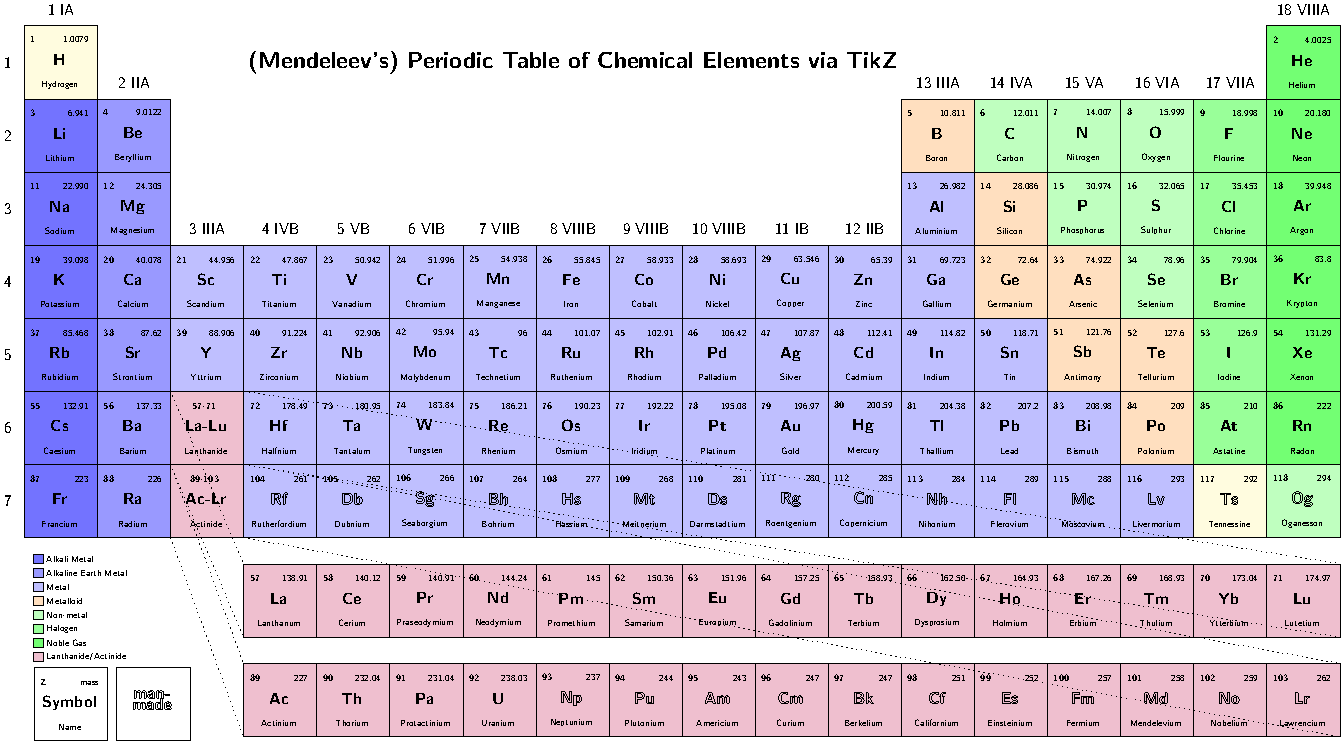
\includegraphics[scale = 1, angle = 90]{gfx/Periodic_table2017}